\section{Software Design}
\subsection{Introduction}
The HYBRID repository is a collection of models and workflows used to assess the technical and economic feasibility of different integrated energy systems. The purpose of the software is to allow the user to design process models quickly and efficiently for use within a technoeconomic analysis. The models are to be designed with the goal of interoperability and “plug and play” design in mind. This design philosophy allows users to quickly create and test new integrated energy systems, control schemes, and energy offtake opportunities and pathways. 

In addition to the high fidelity modelica models the HYBRID repository provides basic workflows that allows direct integration with the Risk Analysis Virtual Environment (RAVEN) code developed at INL and it’s plugins the Heuristic Energy Resource Optimization Network (HERON) and the Tool for Economic AnaLysis (TEAL) packages. Through the integration of these different packages and repositories complete grid analysis and systemwide optimization can be achieved. 

\subsection{Hybrid Repository Structure}
The HYBRID Repository structure is illustrated in Figure 1 where the components are:

\begin{itemize}
\item \textbf{\textit{Models}}: Folder containing the Modelica/Dymola models and future location of new RAVEN workflows generated.
\item \textbf{\textit{doc/user\textunderscore manual}}: Folder containing the user manual for the repository
\item \textbf{\textit{archive}}: containing legacy workflows from previous externally released milestones.
\item \textbf{\textit{TRANSFORM library}}: Submodule of the Oak Ridge National Laboratory (ORNL) based TRANSFORM library that is used as the base models for many of the integrated energy systems models
\item \textbf{\textit{raven}}: submodule linking to the RAVEN (\cite{RAVENuserManual}) repository
\item \textbf{\textit{scripts}}: containing the dymola\textunderscore launcher and the tools for loading Modelica/Dymola outputs into a Python environment
\item \textbf{\textit{tests}}: containing all the tests that are automatically executed by the Continuous Integration system and executable, locally, running the command “run\textunderscore tests.”
\end{itemize}

Within the \textbf{\textit{Models}} folder there are two subfolders \textbf{\textit{NHES}} and \textbf{\textit{RAVEN\textunderscore WORKFLOWS}}. The RAVEN\textunderscore WORKFLOWS folder is empty and is where future RAVEN\textunderscore WORKFLOWS used in techno-economic analysis will be placed. The NHES folder contains all the Modelica models ranging from Gas Turbines to Nuclear power plant and all the associated subsystems. The doc/user\textunderscore manual folder contains the user manual for the HYBRID repository. The archive folder contains the models executed for two 2017 milestones. The \textbf{\textit{TRANSFORM}} submodule is a library of Modelica models created by ORNL in conjunction with the NHES library that is used as the base models for many of the integrated energy systems developed within the NHES library. The \textbf{\textit{TRANSFORM}} submodule is updated on a six month basis and all regression tests are run to ensure none of the models are broken between updates. The raven submodule is a link to the RAVEN repository and is updated frequently to ensure all the latest optimization and processing capabilities are available. The \textbf{\textit{scripts}} folder contains files to allow the automatic launching of Dymola for use within the regression system. Additionally, it holds a folder called testers that contains all the files used to enable the .mat differ used within the regression system ROOK. Then the final folder is tests which contains all the tests that are automatically executed by the Continuous Integration system. Within the \textbf{\textit{tests}} folder there are \textbf{\textit{dymola\textunderscore tests}} and \textbf{\textit{raven\textunderscore tests/train}}. The dymola\textunderscore tests contains all of the dymola regression tests while the raven\textunderscore tests/train contains all of the raven tests that may need to be added as additional raven workflows are added to the Hybrid repository. The repository structure is evolving, but the current topology of the folders will stay the same. 
\begin{figure}[hbtp]
\centering
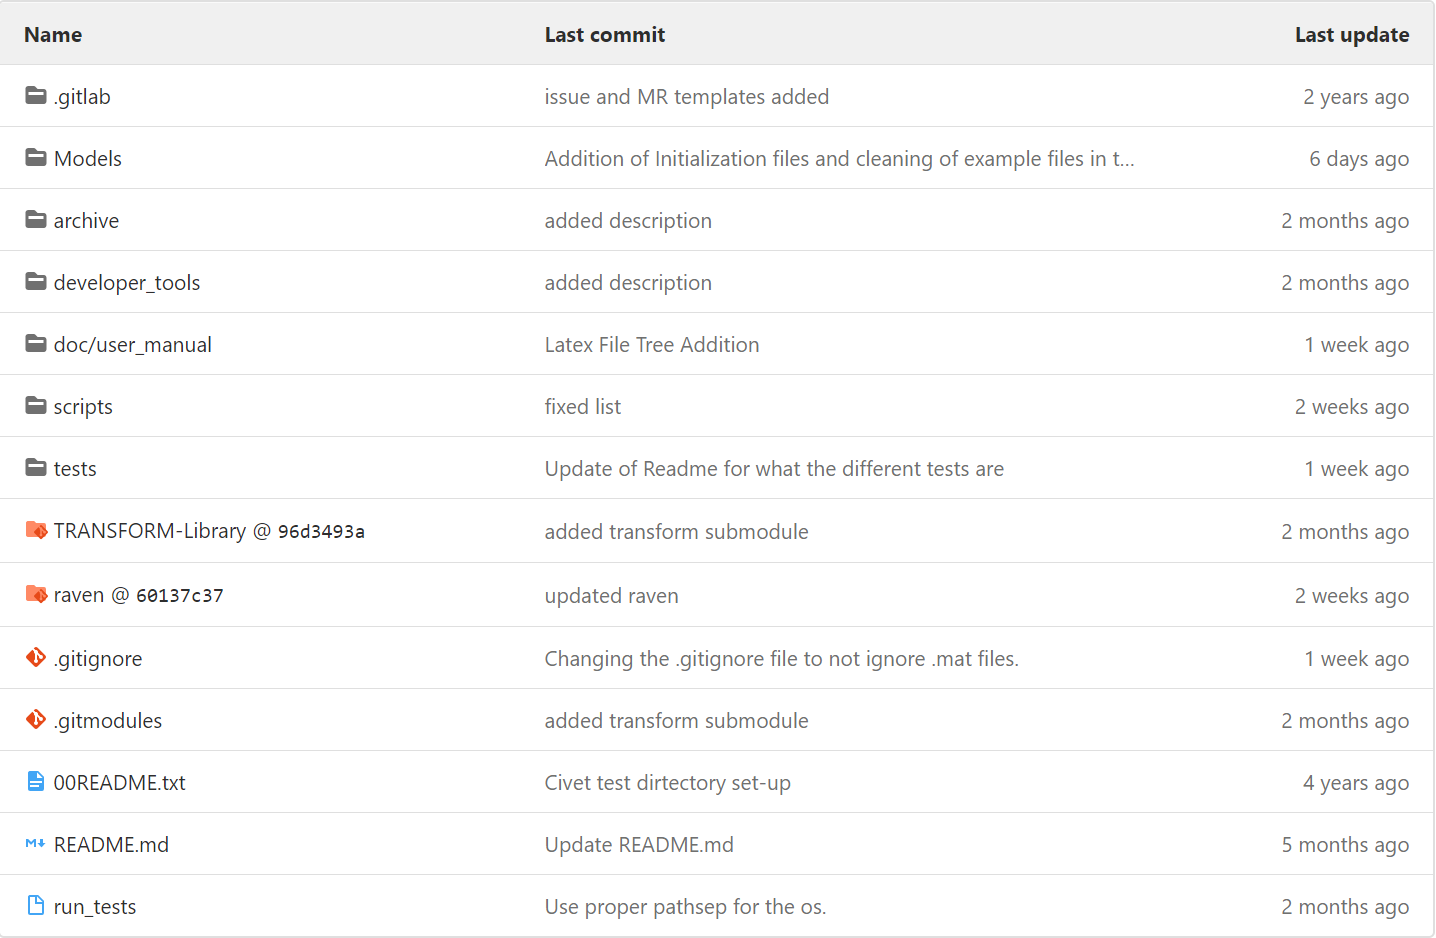
\includegraphics[scale=0.4]{pics/Repository_Structure.png}
\caption{Structure of the HYBRID repository.}
\end{figure}

\subsection{Regression Test System}
HYBRID a repository that contains a series of Modelica models capable of producing potential integrated energy system configurations. To test these models the RAVEN based regression system ROOK has been utilized. This testing system has been linked with the Continuous Integration tool to automatically test the models when new modifications are added to the repository. To do this RAVEN has been sub-moduled within HYBRID. 

\subsubsection{Dymola Regression Tests}
ROOK operates via a basic testing harness. The testing harness includes a “tests” file that contains the tolerance limits, a gold folder with a gold test file, a simulation file to run, a file with which to launch the simulation, and a directory of tests to run. Since the models to be run are Modelica models within the Dymola simulation platform a dymola\textunderscore launcher file was created to automatically run Dymola via the command line interface. For Modelica models the gold file is checked via a .mat file differ that has been created within the ROOK testing harness. This .mat differ checks all variables created by the test and compares them with an earlier version of the system. If the new .mat file is within a specified “tolerance” then the testing harness comes back with a clean pass.  A series of Modelica tests have been added to test the system-level interactions in the Nuclear Hybrid Energy Systems (NHES) Modelica repository and the collection of regression tests will continue to grow as the number of models and model uses grows.

\subsubsection{Raven "Hybrid Specific" Regression Tests}
In addition to the Modelica testing conducted by ROOK additional RAVEN specific tests are run. These raven tests are of workflows that are specific to hybrid energy system workflow generation. HYBRID is designed to be able to provide a techno-economic assessment of different integrated energy systems. As part of this HYBRID includes the generation of RAVEN workflows capable of implementing stochastic time series of wind, solar, and electric price data created via the Auto Regressive Moving Averages (ARMAs) algorithms within RAVEN into a workflow that can then be integrated into the Modelica models. The creation of these ARMAs using data held within the HYBRID repository is maintained using the ROOK system. 


